\documentclass[12pt]{report}
\usepackage[a4paper, left=0.5in, right=0.5in, top=0.5in, bottom=0.5in]{geometry}
\usepackage{xcolor}
\usepackage{amsmath}
\usepackage{amsthm}
\usepackage{amssymb}
\usepackage{amsfonts}
\usepackage{algpseudocode}
\usepackage{mathtools}
\usepackage{xcolor}
\usepackage{float}
\usepackage{framed}
\usepackage{listings}
\usepackage{graphicx}
\usepackage{subcaption}
\usepackage{tikz}
\usepackage{emoji}

\lstset{basicstyle=\ttfamily,
  commentstyle=\color{red},
  keywordstyle=\color{blue},
  %basicstyle=\footnotesize,
  frame=lines,
  numbers=left,
  stepnumber=1,
  showstringspaces=false,
  tabsize=1,
  breaklines=true,
  breakatwhitespace=false,
}
\usepackage{hyperref}
\hypersetup
{
    colorlinks=true,
    linkcolor=blue,
    filecolor=magenta,
    urlcolor=cyan,
    pdftitle={\Huge \textbf{CS218 Solutions NetworkFlow}},
    pdfpagemode=FullScreen,
}
\usepackage[utf8]{inputenc}
\usepackage{graphicx}
\usepackage{longtable}
\usepackage{multirow}
\usepackage{enumitem}
\setlength{\parindent}{0pt}

\begin{document}
\subsection*{\Large\bfseries NetworkFlow}
\begin{enumerate}[label=\textbf{\arabic*.}]

  \item We can do a modified Dijkstra's algorithm here. We'll recursively compute the bottleneck for every single node in our graph.
  The base case is vertex $s$ itself, where there's no bottleneck really so we'll just keep it as $\infty$. Now let's say we have a 
  set of nodes $S$ for which we have already computed all the bottlenecks. Now observe the edges of the cut $(S, G-S)$. If have an 
  edge $uv$, we can say $bottleneck(v) \geq \min(bottleneck(u), C_{uv})$ because we can just go to $u$ in the optimal path, and then 
  get to $v$ using this edge. How we plan to expand our cut, is by looking at the max bottleneck we get from this inequality, i.e.
  look at the max of this term $\min(bottleneck(u), C_{uv})$ for all edges in the cut, and we add this vertex $v$ to $S$ now, and 
  we have found $bottleneck(v)$. But how are we sure this is the most efficient way to get to $v$? Firstly by the definition of our 
  algorithm, this is the best route we can get if we directly want to go from some vertex in $S$, to $v$. And there can't be any path
  exiting the set $S$ and going to $v'$, and then $v'$ to $v$. Because $bottleneck(v') \leq bottleneck(v)$, $v$ by definition was the 
  most optimal way to exit $S$. So by the time we go to $v'$, and then we get from $v'$ to $v$, we can't have some bottleneck greater
  than just directly going to $v$. So we just keep adding vertices to our set $S$ till we finally take $t$ itself.

  \item Not sure how to think of this, just got this example online \emoji{grinning-face-with-sweat}.
  
  \begin{figure}[H]
    \centering
    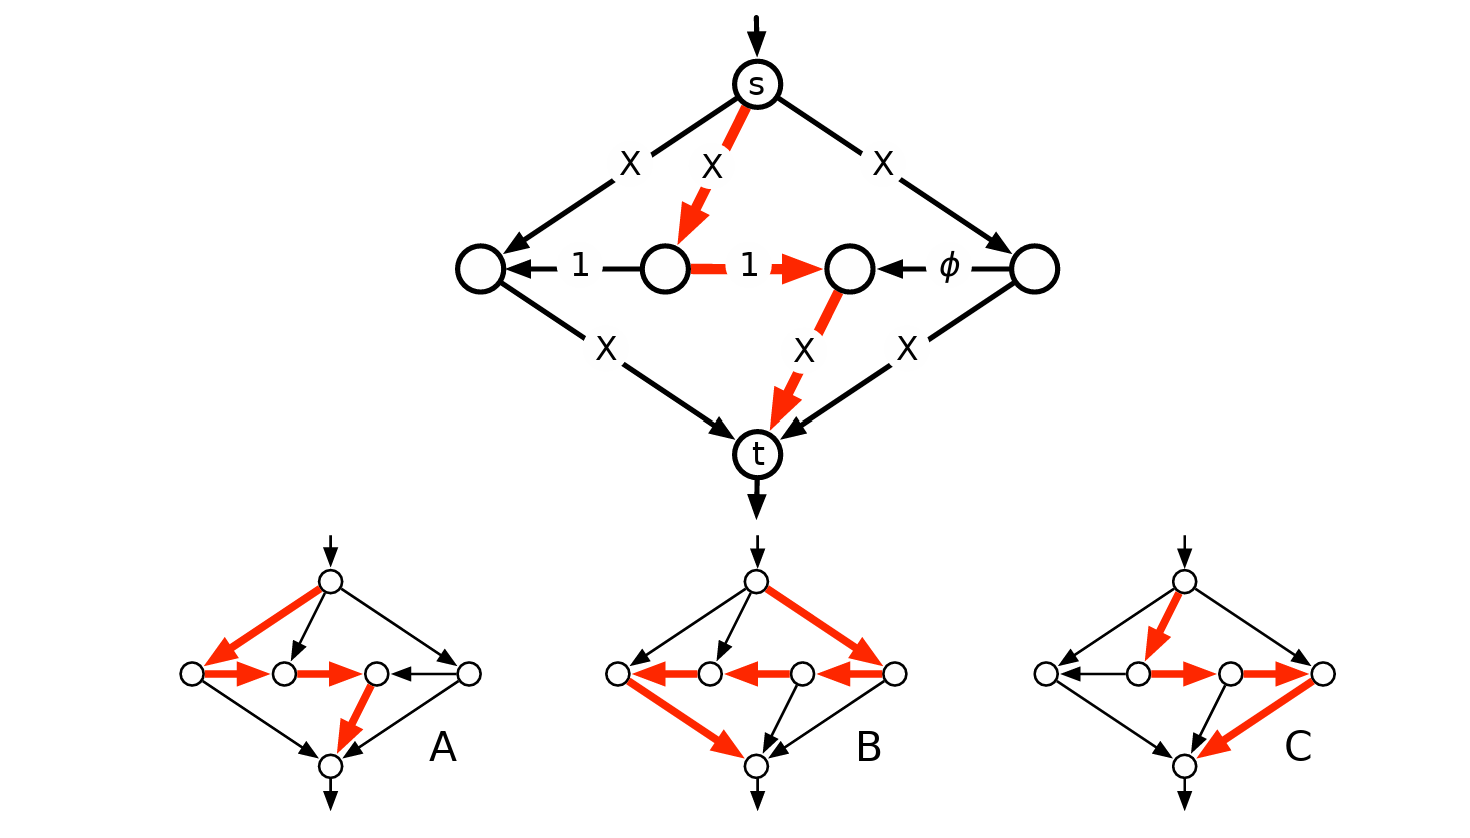
\includegraphics[width=0.5\textwidth]{IrrationalCapacities.png}  
  \end{figure}

  $X$ here is some large number, take it as 100 or something, and $\phi$ is the golden ratio, $\frac{\sqrt{5} - 1}{2}$. 
  For this version of golden ratio $1 - \phi = \phi^2$ There are 3 residual paths we will keep using, $A$, $B$ and $C$. 
  Let's say the first path chosen is the top one, and the residual capacities in the 3 middle edges from left to right 
  are now $1, 0, \phi$ respectively. We will inductively prove that they will be $\phi^{n-1}, 0, \phi^n$ after a series of operations. 
  Now assume it's true for $n=k$, we'll get it to $n = k+2$.
  
  \begin{itemize}
    \item Push along path $B$, adding $\phi^k$ flow. The capacities become $\phi^{k-1} - \phi^k = \phi^{k+1}, \phi^k, 0$
    \item Push along path $C$, adding $\phi^k$ flow. The capacities become $\phi^{k+1}, 0, \phi^k$
    \item Push along path $B$, adding $\phi^{k+1}$ flow. The capacities become $0, \phi^{k+1}, \phi^k - \phi^{k+1} = \phi^{k+2}$
    \item Push along path $A$, adding $\phi^{k+1}$ flow. The capacities become $\phi^{k+1}, 0, \phi^{k+2}$
  \end{itemize}

  So if we keep repeating the above operations, how much flow are we adding? Initially we had a flow of 1, total flow we get is 
  
  \[ 1 + \sum_{k=1}^\infty (\phi^k + \phi^k) = 1 + \frac{2}{1 - \phi} =  4 + \sqrt{5} \]

  But this is clearly not the max flow, we could have just made a flow in the left most path and right most path, and path $B$, 
  getting a flow of $2X + 1$ which for large $X$ is definitely more than $4 + \sqrt{5}$.

  \item As the hint says, we will first choose $\triangle = \sum_e c_e$. And since we want some logarithmic time complexity, at each 
  point where we can't increase the max flow, we will half the value of $\triangle$. So we will have some $\log(\sum_e c_e)$ iterations
  in the outer loop. But we aren't done lol, we have to bound the time taken for each iteration in the loop, if each iteration just
  takes $\sum_e c_e$ time, our method is useless. So let's think a bit more.
  
  During some iteration where we only look at residual edges above $\triangle$, we can say on each iteration in the inner loop, the 
  max flow will increase by at least $\triangle$ (as all residual edges can be increased by at least this much, when we find a new path
  from $s$ to $t$). This fact will be useful in bounding the number of iterations for each value of $\triangle$.

  Now let's observe the flow, and the min cut in the residual graph at the end of some iteration of $\triangle$. Choose $A$ to be the
  vertices reachable from $s$ in the residual graph, and $B$ to be the rest of the vertices. Now in the normal max flow min cut algorithm, 
  we know that $c(A,B)$ will be equal to the flow, but here it isn't the case because we ignore edges with lesser capacities, but we will 
  still try to make an inequality. Look at some edge $e$ from $A$ to $B$. We can say $f(e) > c_e - \triangle$, else there's an edge in the 
  residual graph with more capacity than $\triangle$ in the cut. Similarly for each edge in $B$ to $A$, $f(e) < \triangle$, else there's a 
  backward edge in our residual graph from $A$ to $B$ with capacity at least $\triangle$. So what does this basically mean? For each edge 
  we neglected in the cut from $A$ to $B$, each of them can increase the max flow from $A$ to $B$ i.e. $c(A, B)$ by at most $\triangle$.

  Mathematically speaking, 
  \begin{align*}
    flow &= \sum_{e:A \rightarrow B} f(e) - \sum_{e:B \rightarrow A} f(e) \\
    &> \sum_{e:A \rightarrow B} (c_e - \triangle) - \sum_{e:B \rightarrow A} \triangle \\
    &= \sum_{e:A \rightarrow B} c_e - \sum_{e:A \rightarrow B, B \rightarrow A} \triangle \\
    &\geq c(A,B) - m \triangle
  \end{align*}
  where $m$ is the total number of edges in the graph.

  And we know that $maxflow \leq c(A,B)$ so $flow > maxflow - m \triangle$. This is a pretty powerful result, because in the next iteration 
  $\triangle$ becomes $\triangle/2$ and each iteration at this threshold increases the flow by at least $\triangle/2$, so there'll be at most 
  $2m$ iterations, cause $flow + m \triangle$ is already bigger than maxflow. So we have a result that each iteration has a maximum of $2m$ inner
  iterations, which is a term independent of $\sum_e c_e$. So now we're done, we got a time complexity proportional to $\log(\sum_e c_e)$
  We don't have to worry about the inner iterations being depending on this summation, each one of them is just finding a path from $s$ to $t$,
  actually our overall time complexity is $O(\log(\sum_e c_e) \times m \times m)$.

  \item If the question was find minimum number of edges to disconnect, it becomes much easier. We just make each edge have a capacity of 1, and find
  the max flow. Why does this work? Firstly if the max flow was $k$, you have $k$ edge disjoint paths from $s$ to $t$. You need to delete at least 1 
  edge from each path to disconnect $s$ and $t$, so minimum number of edges to disconnect $\geq k$. You also have a cut with capacity $k$ which means 
  there are exactly $k$ edges from $A$ to $B$ in the cut. Remove all these edges and you disconnect $A$ and $B$, which disconnects $s$ and $t$, 
  so $k$ is in fact possible. But anyways, we need to find minimum number of vertices to disconnect.
  
  Since we somehow need to make sure each vertex is used only once in the flow instead of each vertex, the idea is to break each vertex $v$ 
  into $v_1$ and $v_2$, acting like arrival and departure vertices. For each edge $uv$ in the original graph we draw an edge of infinite capacity
  from $u_2$ to $v_1$. And for each vertex $v$ we add an edge of capacity 1 from $v_1$ to $v_2$, this seems like it will ensure each vertex is `used'
  only once. We can say deleting a vertex $v$ is equivalent to just deleting the edge $v_1 v_2$, cause there's no other way to arrive at $v$ 
  and depart from $v$ in our graph. Now if our max flow was $k$, we have $k$ vertex disjoint paths from $s$ to $t$, requiring at least $k$ deletions
  of vertices. Similarly you have a min cut of capcity $k$, and edges in the cut must all have capacity 1, which are edges of type $v_1 v_2$. We
  just delete all such vertices $v$, which would definitely disconnect $s$ and $t$.

  \item Say we have TAs $T_1, \dots, T_n$. And courses $C_1, \dots, C_k$ each demanding $d_1, \dots, d_k$ TAs. All $T_i$'s and $C_j$'s will be nodes 
  of our graph. We draw a directed edge from $T_i$ to $C_j$ with capacity 1 if TA $T_i$ is eligible to take course $C_j$ and its flow value will
  indicate if $T_i$ is assigned course $C_j$. We connect $C_j$ to a sink
  $t$ with an edge of capacity $d_j$, and its flow will denote the number of TAs assigned to that course. We draw an edge from source $s$ to $C_i$
  with capacity 1 to make sure that the TA takes maximum 1 course\footnote{KarGo \emoji{clown-face}}, and its flow value denotes if the TA has 
  been selected for some course. And that's it, we check the max flow from $s$ to $t$ and check if it's equal to $d_1 + \dots + d_k$. This is possible 
  if and only if every $C_j t$ edge had flow $d_j$, and this is only possible if we found $d_j$ edges to $C_j$ with flow value 1 coming from different 
  TAs. Converse is easy to show, if we have a suitable TA allocation we can construct a flow equal to $d_1 + \dots + d_k$.

  \begin{figure}[H]
    \centering
    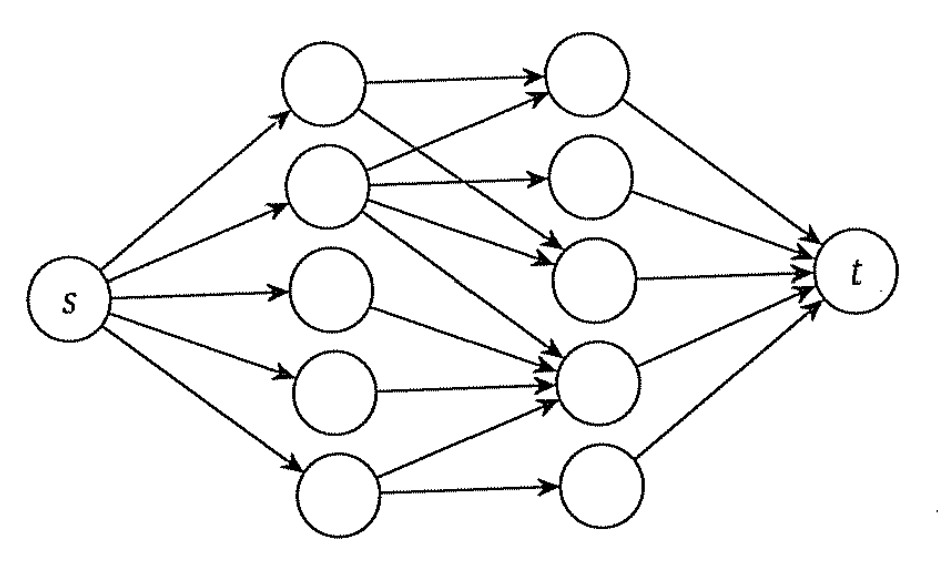
\includegraphics[width=0.5\textwidth]{TAallocation.png}  
  \end{figure}

  Let $(A, B)$ be the minimum cut of this graph. Let $X, X'$ be the TA's in $A$, $B$ respectively. And $Y, Y'$ be the courses in $A$, $B$ 
  respectively. We are going to prove that $Y'$ is a set of courses for which the total number of TAs eligible for them is less than the demand.
  Let's see what all edges are in the cut. Firstly there are edges from $s$ to all of $X'$, so the capacities sum to $|X'|$. Then there are edges
  from $X$ to $Y'$, we don't know how many, and there are edges from $Y$ to $t$ which sum to $\sum_{i|C_i \in Y} d_i$. Let's think about how many TAs
  in $X$ and $X'$ are suitable for courses in $Y'$. So for each TA in $X$ suitable for some course in $Y'$ there will at least be 1 edge from the TA 
  to $Y'$. So we can say number of edges from $X$ to $Y'$ is $\geq$ number of TA in $X$ eligible for $Y'$. And trivially, number of TAs eligible for
  $Y'$ in $X' \leq |X'|$. 
  Now we are going to combine all these results.
  
  \begin{align*}
    c(A,B) = maxflow &< \sum_i d_i \\
    \sum_{e:s \rightarrow X'} c_e + \sum_{e:X \rightarrow Y'} c_e + \sum_{e:Y \rightarrow t} c_e &< \sum_{i|C_i \in Y} d_i + \sum_{i|C_i \in Y'} d_i \\
    |X'| + |\{e:X \rightarrow Y'\}| + \sum_{i|C_i \in Y} d_i &< \sum_{i|C_i \in Y} d_i + \sum_{i|C_i \in Y'} d_i \\
    |X'| + |\{e:X \rightarrow Y'\}| &< \sum_{i|C_i \in Y'} d_i
  \end{align*}

  Since the first term is $\geq$ number of TAs in $X'$ eligible for $Y'$, and second term is $\geq$ number of TAs in $X$ eligible for $Y'$, in the end
  we the fact that total number of TAs eligible for $Y'$ is less than demand of TAs for $Y'$.

  \item 
  \begin{itemize}
    \item We construct the chains as follows:, if $r_i$ is matched with $l_j$, we are sure that $i \leq j$, so we place $i$ just before $j$ in the chain
    decomposition, and we do this for every single matching. Is this a well defined chaining? Well $r_i$ can be matched with only 1 node, so it won't 
    be placed before 2 different $j$'s. Similar $l_j$ is paired with only 1 $r_i$ so its previous element is well defined. So at the end of this process
    how many chains do we get? Initially before chaining up anything, all $n$ elements are kind of like in different chains. Each matching we see, we 
    connect 1 chain to another and reduce the number of chains by 1. So if we have $k$ matchings, we'll have $n-k$ chains.
    If $r_i$ is never matched, it isn't before any $j$ so it will be a maximal element in a chain. Similarly if $l_j$ is never matched, it won't be after
    any $i$ so it is a minimal element in a chain.
    \item We just do the same thing backwards. If $i$ is placed directly before $j$ in a chain, we'll match $r_i$ with $l_j$. Why this is a matching,
    is because $i$ can be directly before a unique $j$ and $j$ can only be directly after a unique $i$. The number of $r_i$'s which aren't matched are
    basically the number of minimal elements, which are the number of chains $= k$. So the number of matches is $n-k$.
    \item Now that we've shown that decomposition into to $k$ chains iff matching of size $n-k$, a maximal matching will correspond to a minimal chain 
    decomposition. A maximal matching of size $n-k$ means we can find a chain decomposition of size $k$, and this is minimal as if we find one smaller than 
    $k$, we'll also be able to find a matching greater than $n-k$, which is a contradiction. 
  \end{itemize}

  \item Let $(A,B)$ be some cut with capacity $n-k$. What we are first going to do is to modify our cut by adding more nodes to $A$, without increasing the 
  capacity. Suppose $i < j$ i.e. $l_i r_j$ is an edge, with $l_i \in A$ and $r_j \in B$. We will just move $r_j$ to $A$ from $B$. How does our cut capacity 
  change? We will gain the edge $r_j t$ but we are at least losing 1 edge, which is $l_i r_j$ itself. So overall our cut capacity can't really increase.
  We just keep doing this, add as many $r_j$'s as we can, until none of the $l_i r_j$ edges are part of the cut. Now we claim that, the set of $i$ such that
  $l_i \in A$ and $r_i \in B$ is an antichain. Can $i,j$ in this set be comparable? If $i<j$, $l_i r_j$ will be an edge. 
  We know $l_i \in A, r_j \in B$. But we just extended $A$ such that none of these are part of the cut, so this isn't possible. Now what's the size of our
  antichain? Let's think about the cut capacity which is the number of edges in the cut. $l_i, r_j$ type edges aren't part of the cut, so only possibilities
  are $s, l_i$, and $r_i, t$ type edges. The only $i$ for which neither of them are an edge in the cut is if $l_i \in A$ and $r_i \in B$, which is exactly
  the elements which aren't in our antichain. What about the case where both are in the cut? Doesn't matter, we are just saying there is at least 1 of these 
  edges for every $i$ which isn't in our antichain i.e capacity is at least $n -$ (number of elements in antichain). We also have the fact that capacity is 
  atmost $n-k$. So in the end we get an antichain of size at least $k$.

  This actually proves Dilworth's theorem, as the number of chains we can partition into is exactly equal $n - maxflow = n - mincut$. 
  Say the number of chains is $k$, then the maxflow, and mincut is equal to $n-k$
  And if the mincut is equal to $n-k$, we can find an antichain of size at least $n - (n-k) = k$. We can't do better than $k$, else we'll pick 2 elements in
  the same chain.

  \item We first reverse all the edges of a graph i.e. we draw a directed edge from $i$ to $j$ if $j$ is a prerequisite for $i$. We also give it a capacity 
  of $\infty$. The motivation for this is like follows, as we are reducing this question to a mincut question, we want to make sure that none of these edges 
  are in the cut else we choose a project without its prerequisite, and infinite capacity edges won't ever be part of the mincut. Now we add a source $s$ and
  a sink $t$. If $p_i$ is positive we connect $s$ to $i$ with capacity $p_i$. If $p_i$ is negative we connect $i$ to $t$ with capacity $-p_i$. Because of 
  the infinite edges we know that the mincut will satisfy precedence constraints. 

  \begin{figure}[H]
    \centering
    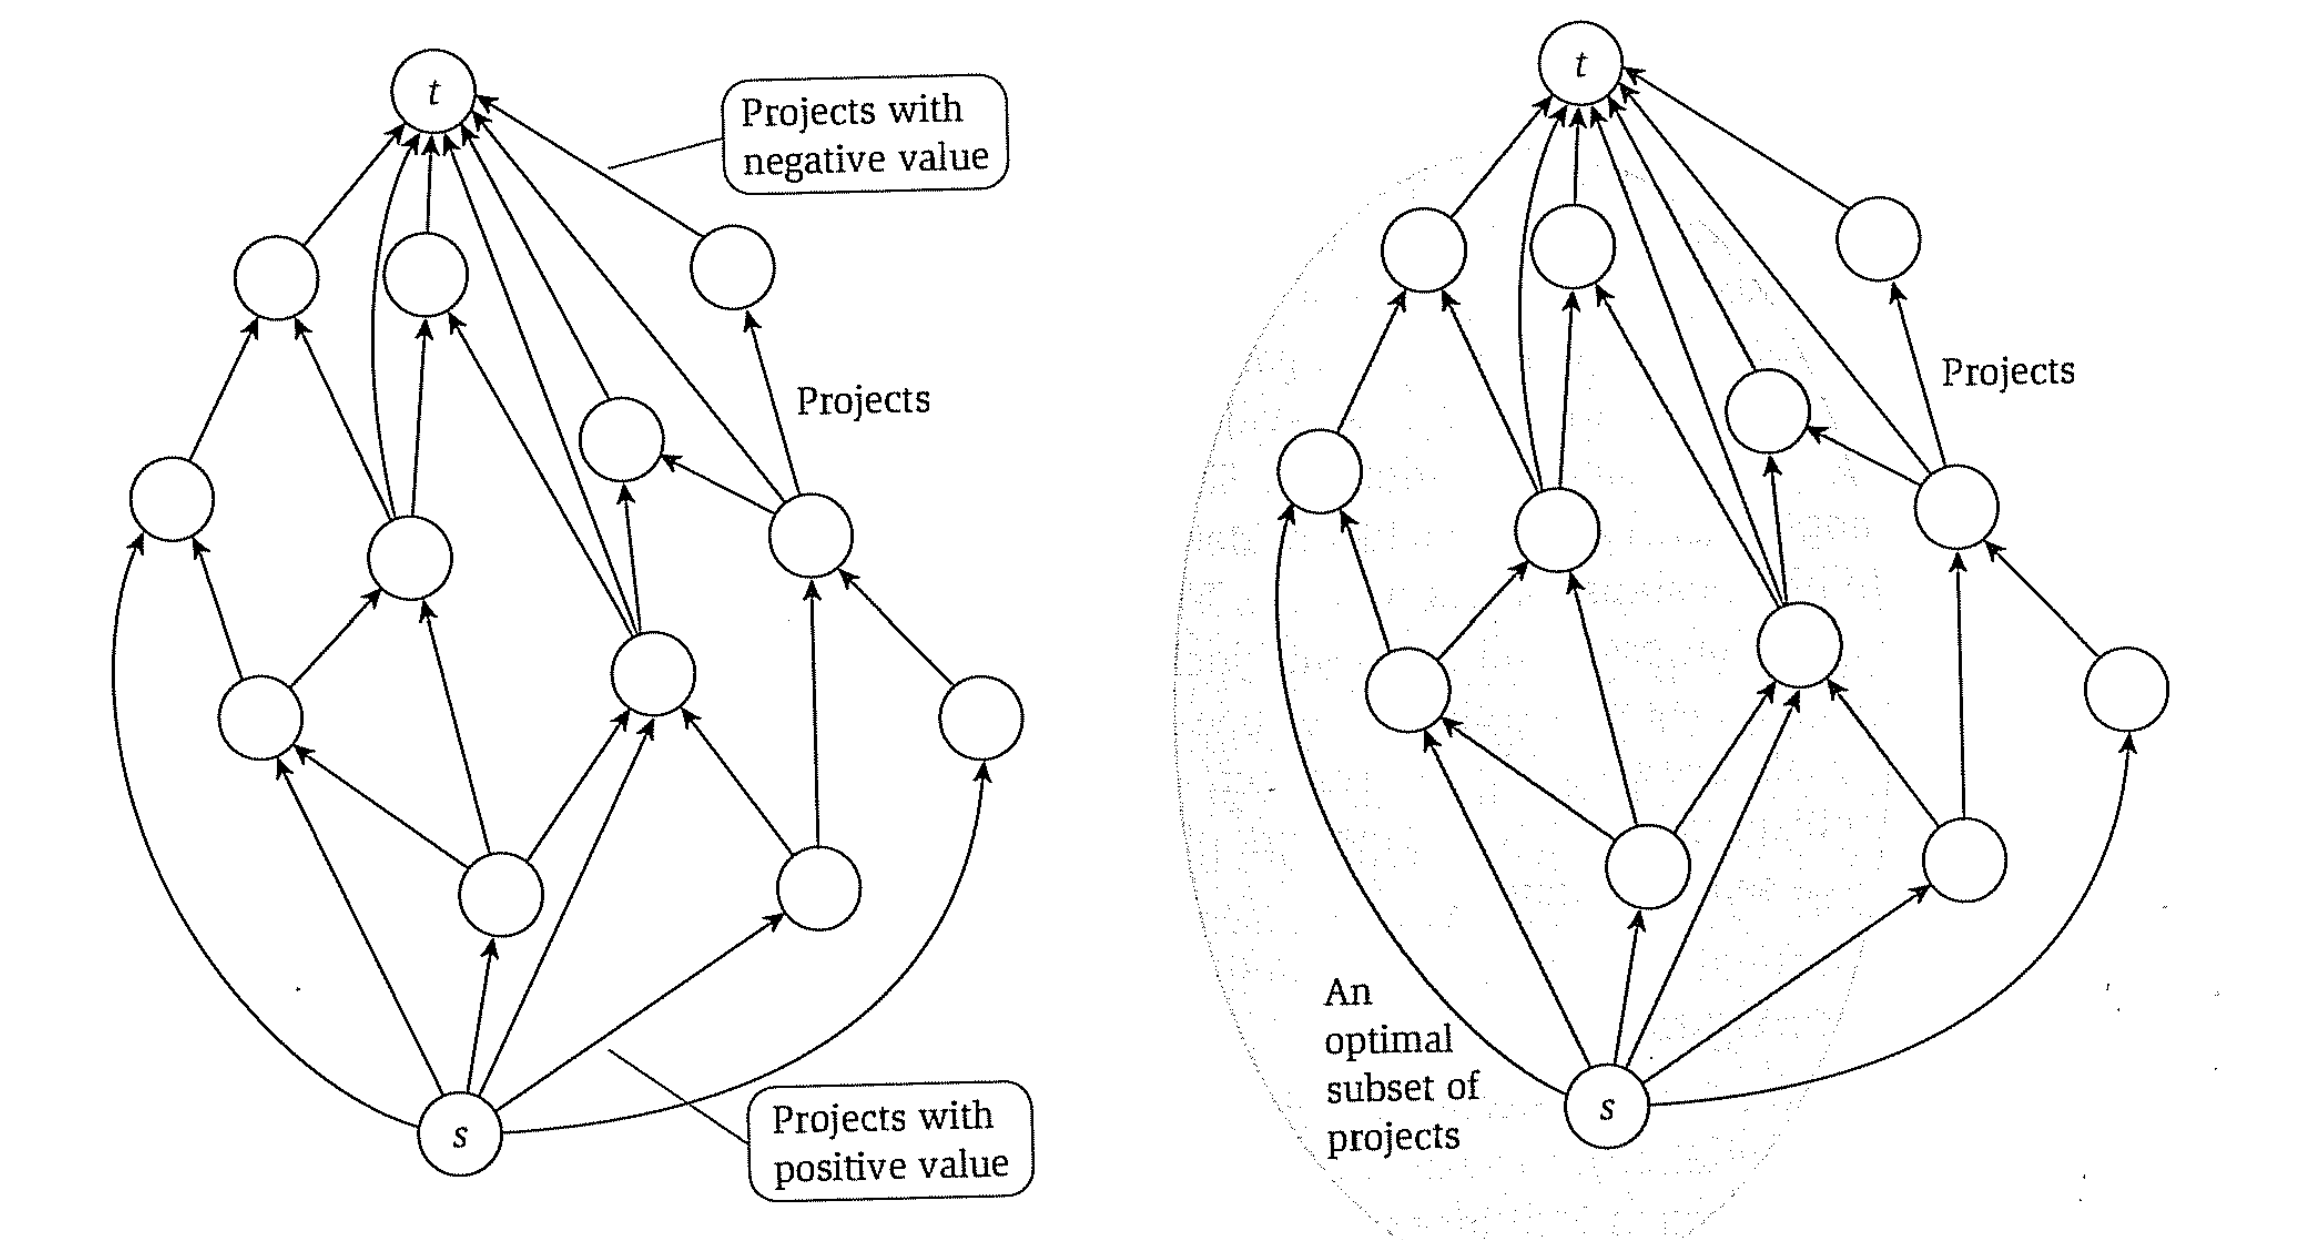
\includegraphics[width=0.8\textwidth]{ProjectSelection.png}  
  \end{figure}

  Now let's look at a random cut $(A,B)$ and try to see what is its capacity. There are $(s,i)$ type edges, whose sum is basically $\sum_{i \in B, p_i>0} c_{si}$.
  There are also $(i,t)$ type edges whose sum will be $\sum_{i \in A, p_i<0} c_{it}$. No infinite type edges will be there in any $A$ which satisfies precedence 
  constraints. The total capacity is hence
  \begin{align*}
    c(A,B) &= \sum_{i \in B, p_i>0} c_{si} + \sum_{i \in A, p_i<0} c_{it} \\
    &= \sum_{i \in B, p_i>0} p_i + \sum_{i \in A, p_i<0} -p_i \\
    &= \sum_{i, p_i>0} p_i - \sum_{i \in A, p_i>0} p_i - \sum_{i \in A, p_i<0} p_i \\
    &= \sum_{i, p_i>0} p_i - \sum_{i \in A} p_i
  \end{align*} 

  The first term is a constant no matter what $A$ is, so if we minimize the cut, we maximize $\sum_{i \in A} p_i$, which is exactly what we want.

  \item We want a conservative estimate i.e we want the maximum number of tigers that we're sure have to exist. Experts have distinguished many $l_i$'s 
  and $r_j$'s, but any pair which isn't represented by an edge could potentially be the same. Since we want to give a conservative estimate, we try to 
  maximise the pairings. First what we do is complement the edges i.e. connect $l_i$'s and $r_j$'s which the experts aren't sure are different. And then 
  find the largest matching possible (can be done by max flow). Our answer is basically $k + m + n \ -$ (maximum number of matchings), as each matching 
  will decrease the answer from $k+m+n$ by 1.
  
  \end{enumerate}
\end{document}